\section{Related Work}
\label{sec: related work}

\begin{figure}[t]
\centering
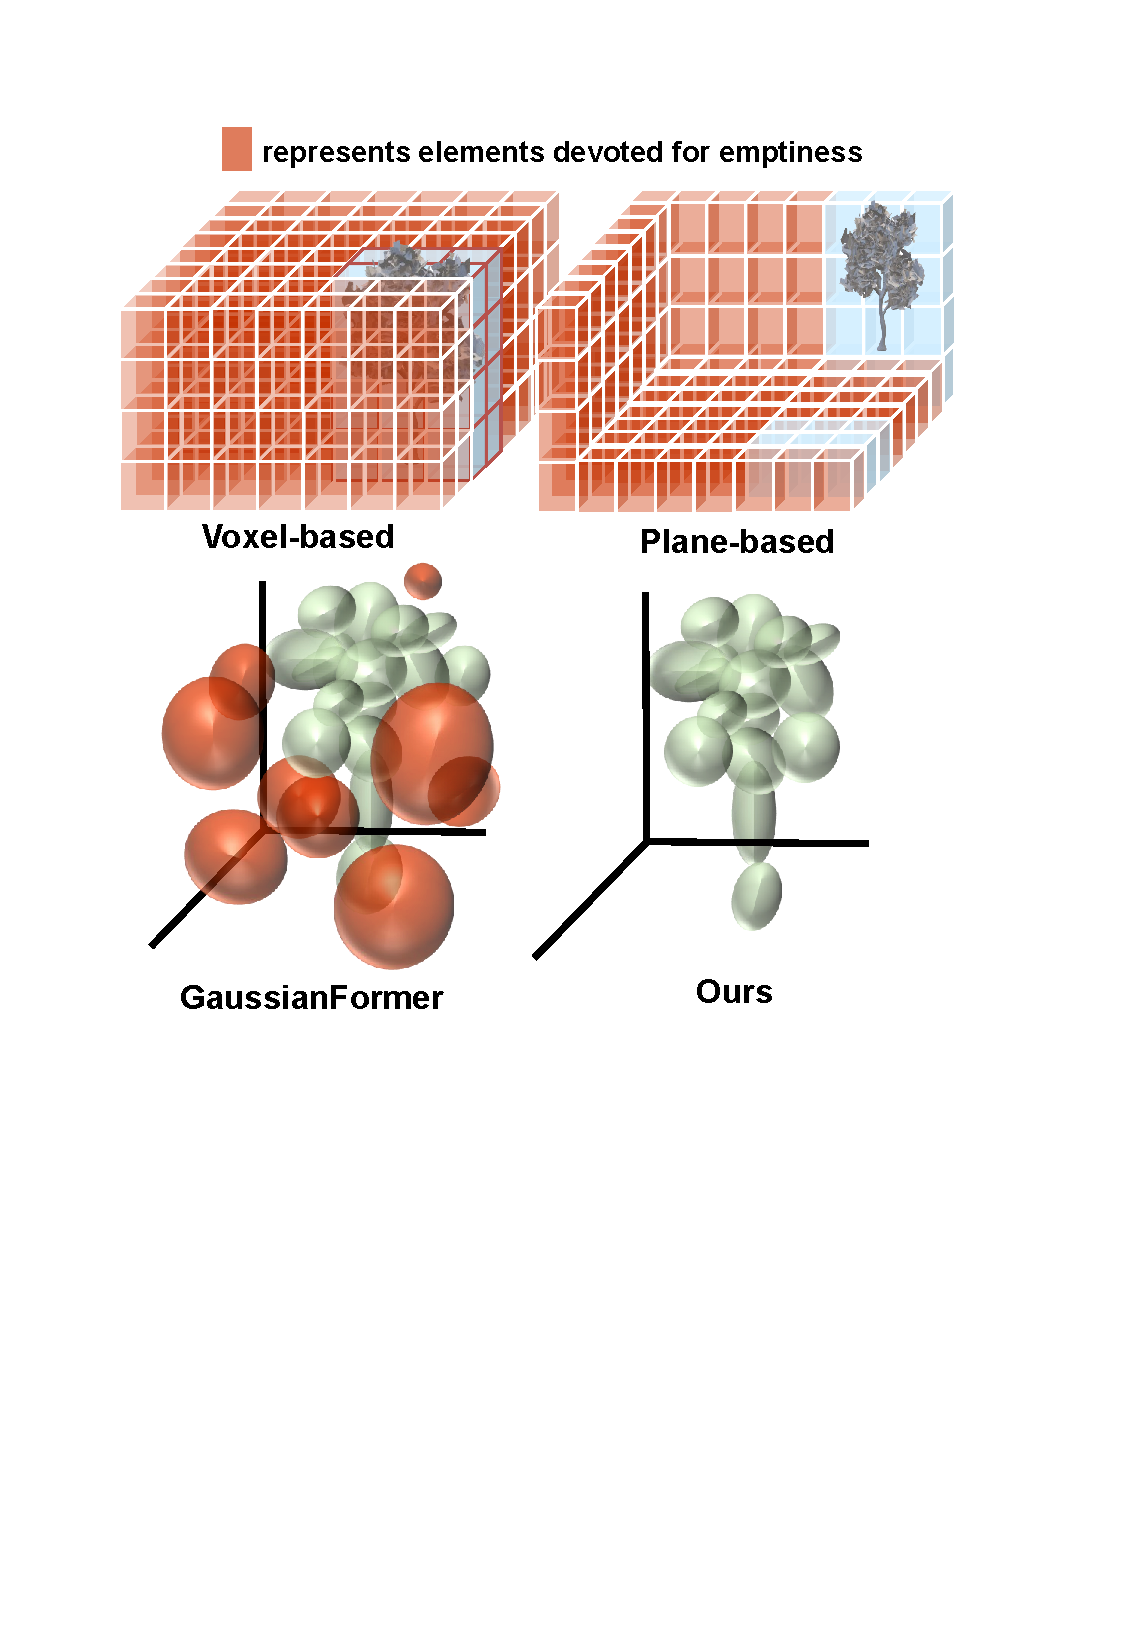
\includegraphics[width=0.95\linewidth]{figures/motivation_1.pdf}
\vspace{-2mm}
\caption{\textbf{Representation comparisons.}
Voxel and plane based representations inevitably incorporate emptiness when modeling the 3D scene.
While GaussianFormer~\cite{huang2024gaussian} proposes 3D semantic Gaussian as a sparse representation, it still suffer from spatial redundancy.
Our method achieves true object-centricity through probabilistic modeling.
}
\label{fig:motivation}
\vspace{-7mm}
\end{figure}


\begin{figure*}[t]
\centering
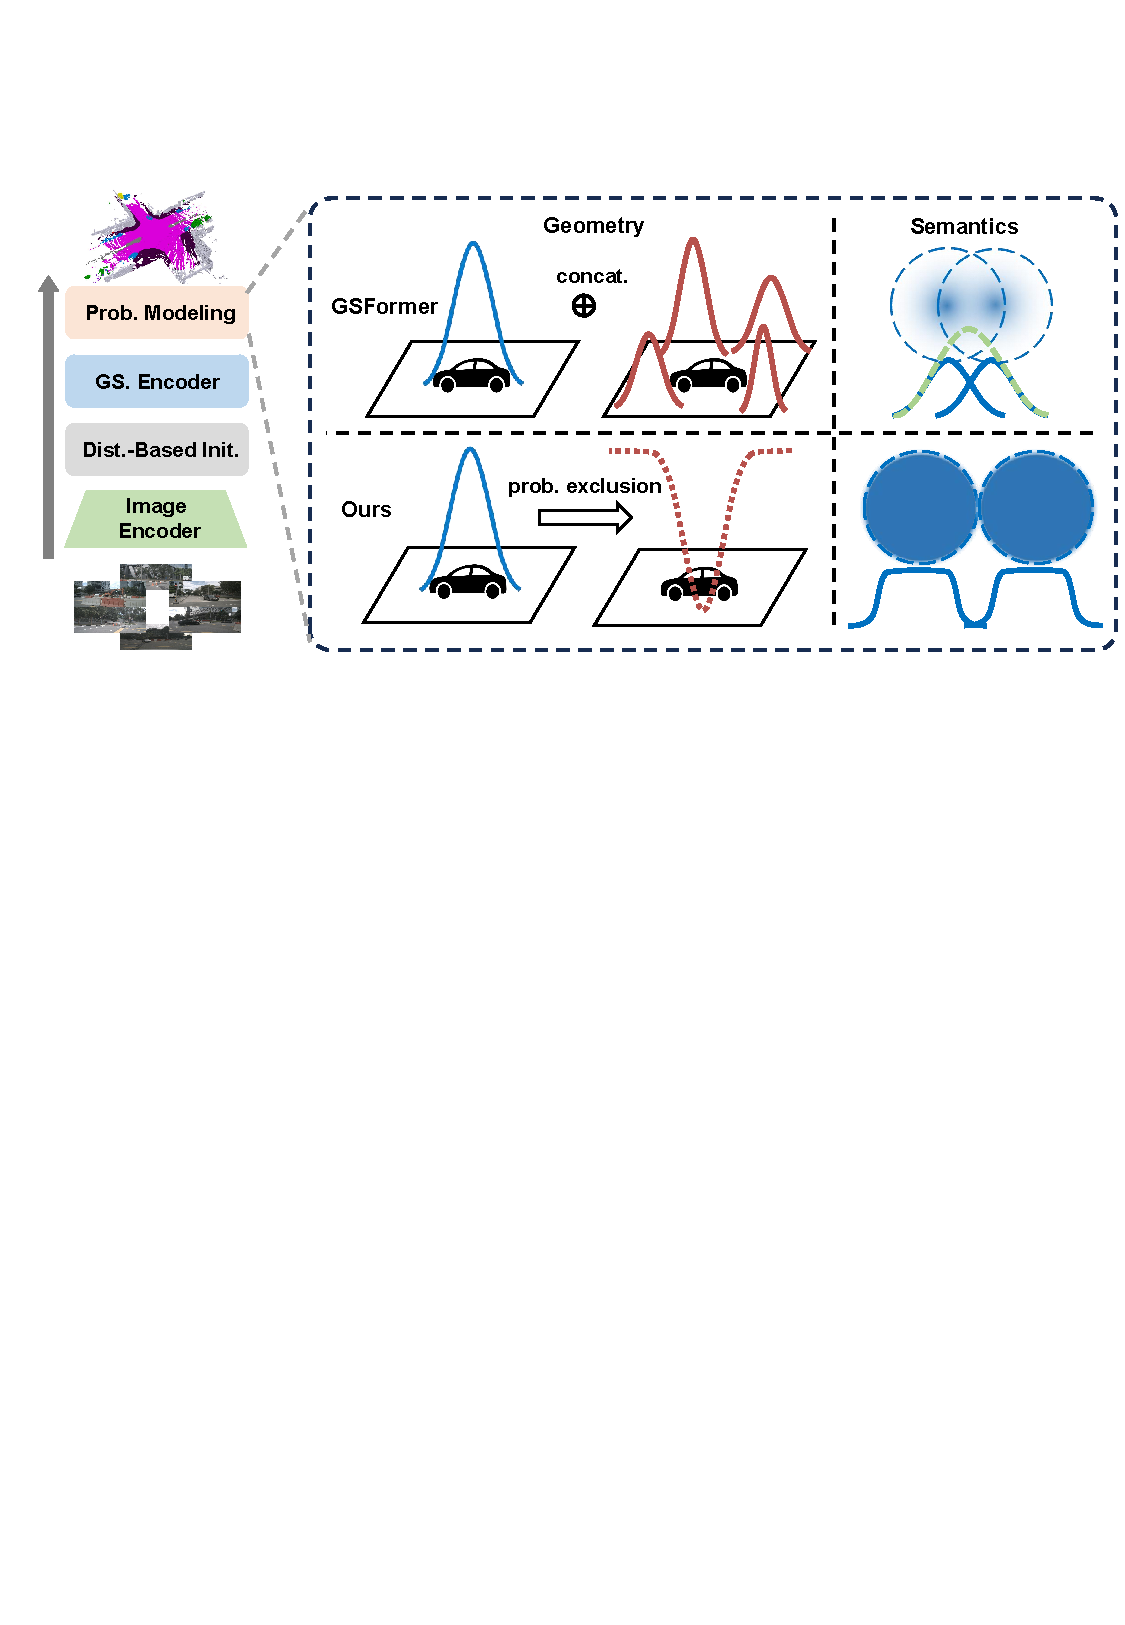
\includegraphics[width=0.95\linewidth]{figures/pipeline_1.pdf}
\vspace{-2mm}
\caption{\textbf{Overall pipeline of our method.}
To achieve probabilistic modeling, we decompose occupancy prediction into geometry and semantics prediction, and approach them separately using probabilistic multiplication and Gaussian mixture model to improve efficiency.
}
\label{fig:pipeline}
\vspace{-6mm}
\end{figure*}



\textbf{3D Semantic Occupancy Prediction.}
3D semantic occupancy prediction~\cite{cao2022monoscene,huang2023tri,tian2023occ3d} has emerged as a promising environment modeling in autonomous driving as it describes driving scenes in a comprehensive manner. 
This task aims to label each voxel in the scene by taking one or more types of sensors as input. 
Two most used sensors are LiDAR and the camera. 
Although LiDAR-based methods perform remarkably well in 3D perception tasks~\cite{cheng20212s3net, liong2020amvnet, tang2020searching, ye2023lidarmultinet, ye2021drinet++, lang2019pointpillars, zhou2018voxelnet, chen2017multi, yan2021JS3CNet, lmscnet, aicnet, 3DSketch, cao2022monoscene}, they possess limitations under bad weather conditions and in detecting distant objects; 
Thus, camera-based approaches have garnered increasing attention~\cite{wei2023surroundocc,yu2023flashocc,li2023fb}. 
Pioneer works in 3D semantic occupancy prediction task adopt dense grid-based representation as a straightforward mean to derive occupancy~\cite{li2023voxformer,wei2023surroundocc,3Chen20193DSS}, then subsequent works turn to sparse object-centric representation~\cite{tang2024sparseocc,lu2023octreeocc,huang2024gaussian} as a solution to the innate problem of redundancy for dense representations. 

\textbf{Grid-based scene representations.}
Plane representations have emerged as competitive representations in scene perception tasks for autonomous driving. 
BEVFormer~\cite{li2022bevformer} is the initiative work of the kind~\cite{huang2021bevdet, li2022bevdepth, philion2020lss, liang2022bevfusion, liu2023bevfusion} that utilizes only camera input and performs comparably well with LiDAR-based methods in detection and segmentation tasks. 
It converts the image feature to the bird's-eye-view (BEV) feature as a unified scene representation, since the information is most diverse at this point of view.
The BEV feature is then used for downstream tasks.
However, the BEV feature is not suitable for 3D occupancy construction as it causes height information to be lost~\cite{wei2023surroundocc}. 
As a generalization of BEV space, TPVFormer~\cite{ huang2023tri} proposes tri-perspective view representation to include also the height information, thus making it more suitable for 3D scenes. 
Another research direction~\cite{wei2023surroundocc, li2023voxformer} adopts voxel-based representation as a more 3D-specific and fine-grained approach, making it favorable for 3D volumetric semantic prediction. 
Nevertheless, these methods utilize dense grid-based representation, which describes each voxel equally regardless of the spatial sparsity of the environment, thus resulting in intrinsic redundancy.

\textbf{Object-centric scene representations.}
To eliminate spatial redundancy inherent in dense representations, many recent works adopt sparse representation~\cite{tang2024sparseocc,lu2023octreeocc,huang2024gaussian}. 
One line of work divides dense grids into partitions where objects present and omits the regions foreseen as empty~\cite{lu2023octreeocc, tang2024sparseocc}. 
However, non-empty regions might be mistakenly classified as unoccupied and eliminated completely from the whole subsequent process. 
Another line of work leverages point representation ~\cite{shi2024occupancysetpoints, wang2024opus} by sampling points within the scene range as queries in the succeeding refinement process; 
Nevertheless, a point has a limited range of depiction as it has no spatial extent. 
An alternative approach, GaussianFormer~\cite{huang2024gaussian}, adopts 3D semantic Gaussian representation, where probability spreads around a mean, allowing more utilization. However, spatial redundancy persists due to no regulation for the Gaussians to not represent emptiness. 
